%\documentclass{beamer}
%\usetheme{Pittsburgh}
\documentclass{scrartcl}

\usepackage[utf8]{inputenc}
\usepackage{default}
\usepackage[procnames]{listings}
\usepackage{graphicx}
%\usepackage[toc,page]{appendix}
\usepackage{caption}
\usepackage{hyperref}
\usepackage{color}
%\usepackage{csvsimple}
\usepackage{float}
\usepackage[T1]{fontenc}



%Bibliogrpahy?
\usepackage{bibentry}
%\nobibliography*
%\bibentry{ }


%Python
\definecolor{keywords}{RGB}{255,0,90}
\definecolor{comments}{RGB}{0,0,113}
\definecolor{red}{RGB}{160,0,0}
\definecolor{green}{RGB}{0,150,0}
\lstset{language=Python,
    basicstyle=\ttfamily\scriptsize,
    keywordstyle=\color{keywords},
    commentstyle=\color{comments},
    stringstyle=\color{red},
    identifierstyle=\color{green},
    breaklines = true,
    columns=fullflexible,
    %Numbering and tabs
    %numbers=left,
    %numberstyle=\tiny\color{gray},
    %stepnumber=2,
    %numbersep=1em,
    tabsize=4,
    showspaces=false,
    showstringspaces=false}

\begin{document}

\title{Scientific Experimentation and Evaluation
}
\subtitle{
Assignment: 4.1}
\author{
  Matin, Maryam \\
  Quignon, Christophe
  %Familyname, Name
}
\date{\today}


\maketitle


\section{Robot design}
%How do you attach the marker
%especially how you mark the stop position and how you ensure identical start positions.
We choose to use the "\href{http://www.damienkee.com/home/2011/8/20/domabot-classroom-robot-design.html}{Domabot}" design in order to minimize the measurement errors. This design has several advantages in this regard:
\begin{itemize}
\item The Motors are directly attached to the brick. Thus the points where distortion can happen are minimized.
\item The center of gravity is very low which increases stability.
\item The track width is big which also increases stability.
\item The free running wheel is rigid and quite narrow. Thus it adds less error by friction or deformation.
\end{itemize}

To mark the endpoints of our measures, we adapted the pen holder  (See Figure~\ref{fig:updown}) to hold the marker. We again can flip the holder up and down.


%UPDOWN
\begin{figure}[H]
\centering
\begin{minipage}{.5\textwidth}
  \centering
  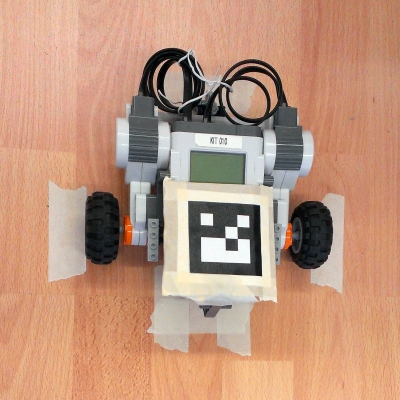
\includegraphics[width=.8\linewidth]{img/top_up.jpg}
  %\caption{}
  %\label{fig:}
\end{minipage}%
\begin{minipage}{.5\textwidth}
  \centering
  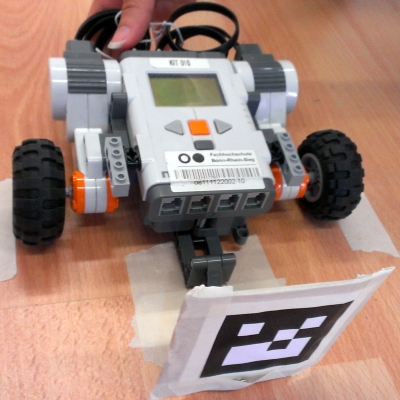
\includegraphics[width=.8\linewidth]{img/front_down.jpg}
  %\caption{}
  %\label{fig:} 
\end{minipage}
\caption{The up and down position of the marker on the robot in starting position.}
\label{fig:updown}
\end{figure}
%Description


\section{Method}
\subsection{Pose of center of motion}
The center of the marker was placed at the center of motion of the robot as seen in Figure\ref{fig:updown} hence the marker tracked the center of motion of the robot.

\section{Documentation}
%how do you ensure correct operation

%camera
\begin{figure}[H]
\centering
\begin{minipage}{.5\textwidth}
  \centering
  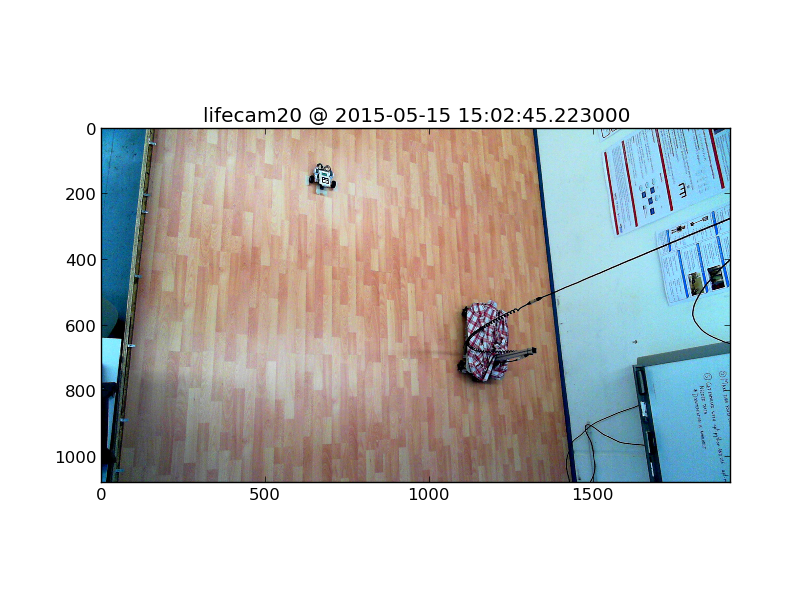
\includegraphics[width=.8\linewidth]{img/marker_up.png}
  %\caption{}
  %\label{fig:}
\end{minipage}%
\begin{minipage}{.5\textwidth}
  \centering
  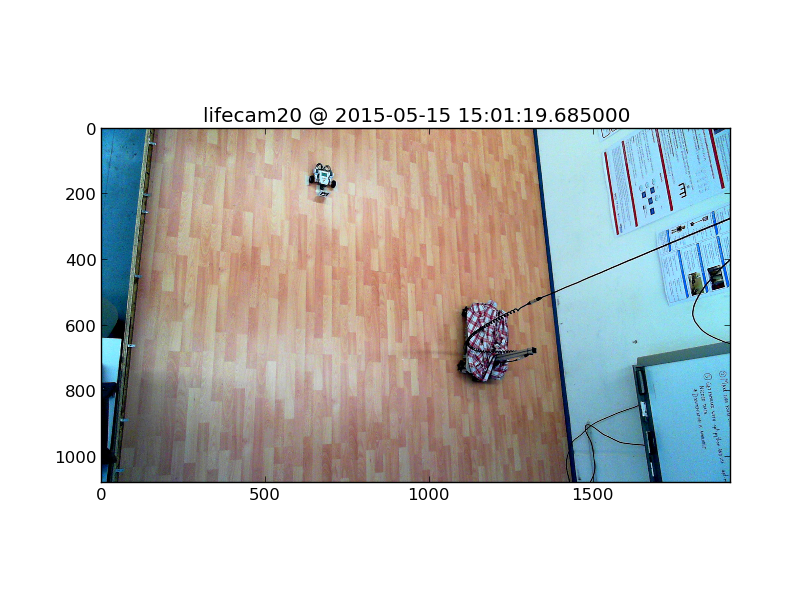
\includegraphics[width=.8\linewidth]{img/marker_down.png}
  %\caption{}
  %\label{fig:} 
\end{minipage}
\caption{The camea view of the robot with marker up(left) and down(right).}
\label{fig:camera}
\end{figure}
%Description

\section{Estimation of pose measurement}
The pose was recorded in roll, pitch and yaw. We only use roll because the robot can not leave the ground. The roll is depicted as the orientation of the triangle in the Figures below.\\
Those figures also show how the measurements have a gap when the marker tracking switched from one camera to another.

\subsection{ahead}
%AHEAD
\begin{figure}[H]
\centering
\begin{minipage}{.5\textwidth}
  \centering
  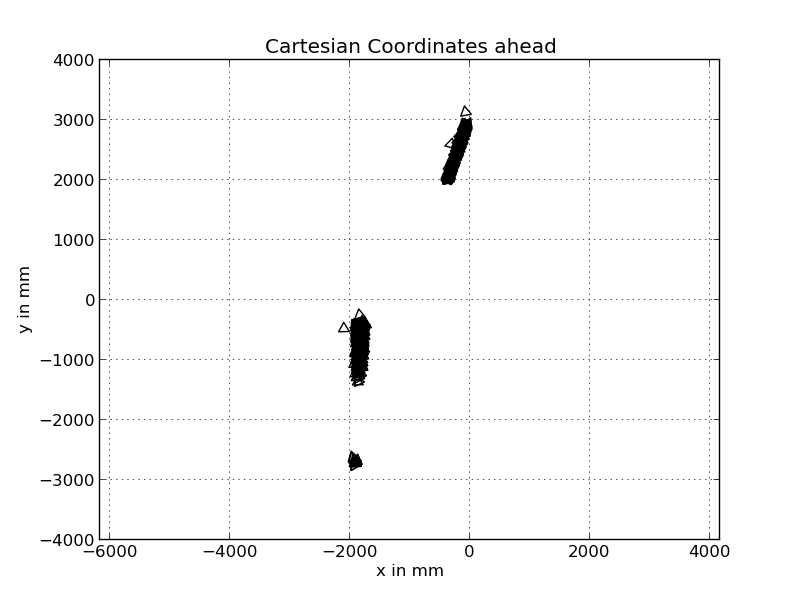
\includegraphics[width=.8\linewidth]{img/ahead.png}
  %\caption{}
  %\label{fig:}
\end{minipage}%
\begin{minipage}{.5\textwidth}
  \centering
  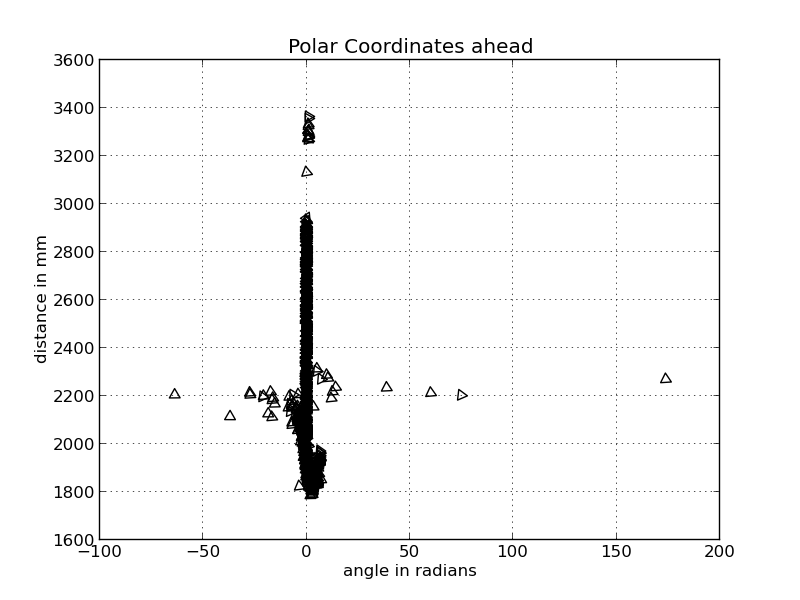
\includegraphics[width=.8\linewidth]{img/ahead_pc.png}
  %\caption{}
  %\label{fig:} 
\end{minipage}
\caption{Recordings of the ahead movements in cartesian and polar coordinates.}
\label{fig:ahead}
\end{figure}
%Description


\subsection{left}
%LEFT
\begin{figure}[H]
\centering
\begin{minipage}{.5\textwidth}
  \centering
  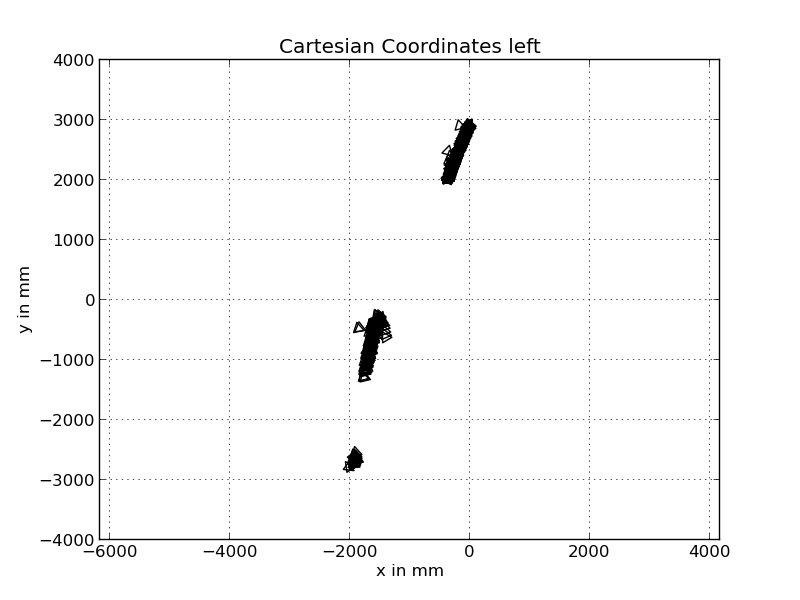
\includegraphics[width=.8\linewidth]{img/left.png}
  %\caption{}
  %\label{fig:}
\end{minipage}%
\begin{minipage}{.5\textwidth}
  \centering
  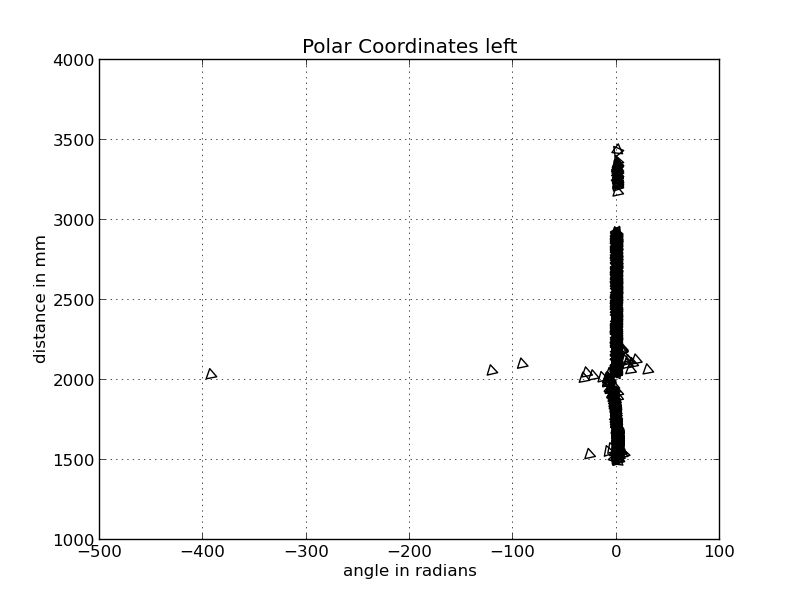
\includegraphics[width=.8\linewidth]{img/left_pc.png}
  %\caption{}
  %\label{fig:} 
\end{minipage}
\caption{Recordings of the left movements in cartesian and polar coordinates.}
\label{fig:left}
\end{figure}
%Description


\subsection{right}
%RIGHT
\begin{figure}[H]
\centering
\begin{minipage}{.5\textwidth}
  \centering
  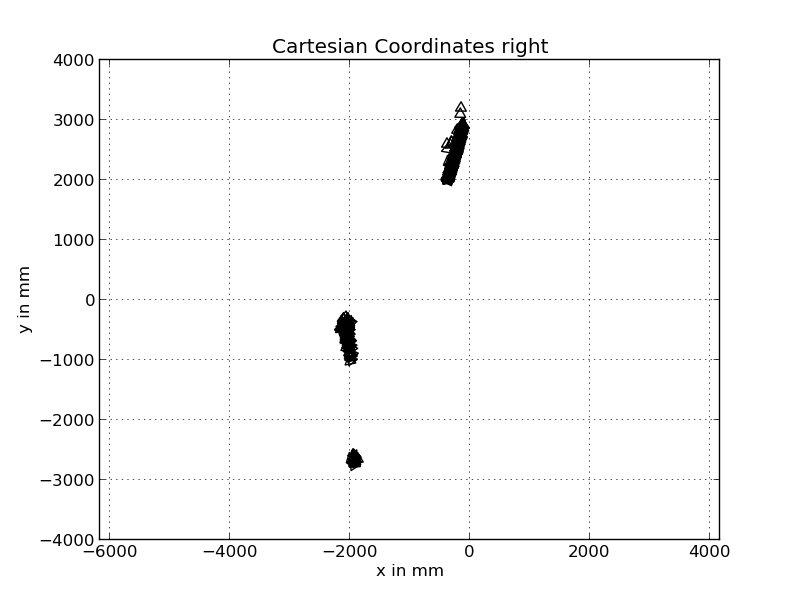
\includegraphics[width=.8\linewidth]{img/right.png}
  %\caption{}
  %\label{fig:}
\end{minipage}%
\begin{minipage}{.5\textwidth}
  \centering
  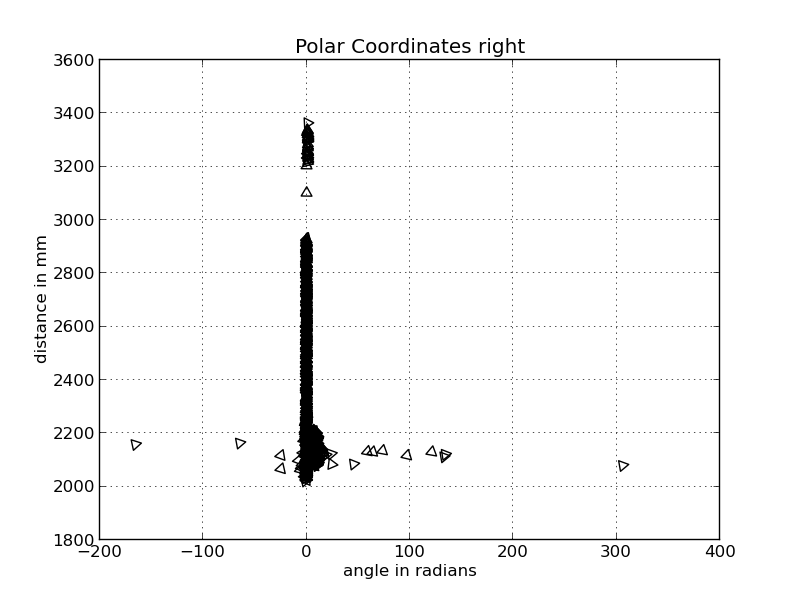
\includegraphics[width=.8\linewidth]{img/right_pc.png}
  %\caption{}
  %\label{fig:} 
\end{minipage}
\caption{Recordings of the right movements in cartesian and polar coordinates.}
\label{fig:right}
\end{figure}
%Description

\subsection{box plots}
The gaps in the recordings made it necessary to not exclude outliers in from the box plots.

%RIGHT
\begin{figure}[H]
\centering
\begin{minipage}{.5\textwidth}
  \centering
  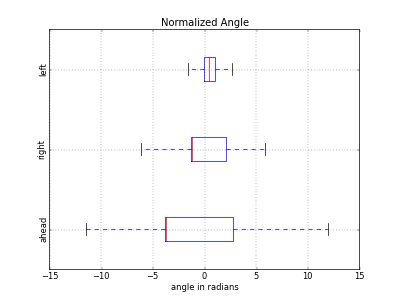
\includegraphics[width=.8\linewidth]{img/BoxplotAngleNorm.png}
  %\caption{}
  %\label{fig:}
\end{minipage}%
\begin{minipage}{.5\textwidth}
  \centering
  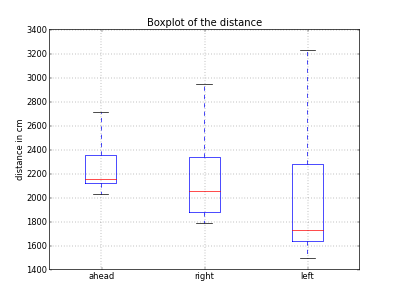
\includegraphics[width=.8\linewidth]{img/BoxplotDistance.png}
  %\caption{}
  %\label{fig:} 
\end{minipage}
\caption{Boxplots of the normed angles and the distances.}
\label{fig:right}
\end{figure}
%Description





\section{Appendix}

\lstinputlisting[language=python]{graphics.py}






%BIBLIOGRPAHY!
\bibliographystyle{plain}%amsalpha
\bibliography{bib.bib}
%\bibentry{}


%COPY AND PASTE FROM HERE

%\begin{enumerate}
% \item
%\end{enumerate}

%\href{link}{text}

%\begin[Language=Python]{lstlisting}
%#PYTHON CODE HERE
%\end{lstlisting}

%\lstinputlisting[language=Java]{ }

%\csvautotabular[separator=semicolon]{data.csv}

%\begin{figure}
% \center
% \includegraphics[width= cm]{img/ }
% \caption{}
%\end{figure}



\end{document}
